\documentclass[12pt,fleqn]{article}\usepackage{../../common}
\begin{document}
Paralel Lineer Cebir Temeli

Satırsal $A^TA$

[5]'te tek makinalı ortamda matris çarpımının nasıl yapılacağını, ve nasıl
görülecebileğini anlattık. Satır bakış açısı, kolon bakış açısı işlendi. Peki
parallel bir ortamda hangi matematik bizi ilgilendirmeli? Mesela $A^TA$'yi ele
alalım. Bu çarpım oldukça önemli çünkü başka sonuçlar için de kullanılabiliyor,
Eşsiz Değer Ayrıştırması (Singular Value Decomposition -SVD-) bunlardan biri.

Büyük Veri ve paralel işlem bağlamında $A^TA$'nin önemli şurada; eğer $A$
matrisi ``uzun boylu ve zayıf'' ise, yani çok miktarda satırı ama az miktarda
kolonu var ise, $m \times d$ diyelim, $A^TA$ çarpımı bize $d \times d$ boyutunda
ufak bir matris verir. Eğer SVD hesabını bu matris üzerinden yapabilirsek,
işimizi kolaylaştırmış oluruz. 

Satırsal olarak $A^TA$ hesabı yapmak için satır satır gezerken her satırın
kendisi ile dışsal çarpımını (outer product) alıp sonuçları toplamak yeterli
[9]. İşlemi daha sözel tarif eden bir açıklama [3]'de bulunabilir.

$A^TA$ ve SVD

$A^TA$ açılımını yapalım [7], bir $A$ için SVD ayrıştırması

$$
A = U \Sigma V^T
$$

olduğuna göre

$$
A^TA =  (U \Sigma V^T)^T  U \Sigma V^T
$$

olacaktır, devam edersek,

$$
= V \Sigma U^T U \Sigma V^T 
$$

$U^T U = I$ olduğu için geri kalanlar

$$
A^TA = V \Sigma^2 V^T 
$$

Peki eşitliğin sağından $V$'yi nasıl çıkartırız? Bir dikgen matris çarpı köşegen
bir matris çarpı o dikgen matrisin devriği bize bir şeyi hatırlatıyor mu?  Evet,
bu bir özdeğer / özvektör hesabına benziyor, [2]'de görüldüğü gibi $A=S\Lambda
S^{-1}$ ayrıştırması da var (birimdik matrislerde tersi alma işleminin devrik
ile aynı şey olduğunu unutmayalım). O zaman $A^TA$'nin öz hesabını yaparsak
oradaki özvektör bize $V$ matrisini verecektir.

$U$'yi elde etmek için basit matris çarpımları yeterli,

$$
A = U \Sigma V^T \to U = A V \Sigma^{-1}
$$

Yani $V$ elde edildikten sonra onunla $A$'yi çarpıyoruz, sonra $\Sigma^{-1}$
ile. $A$ ne kadar büyük olursa olsun onu bir vektör $V$ ile çarpmak hızlı
işler, $\Sigma$ ise köşegen, seyrek bir matristir, onun çarpımı da basittir.

Bu işlemlerin paralel versiyonları için [8, 6] kaynaklarına bakılabilir.

SVD ve öz hesapların benzerliği için alttaki koda bakılabilir,

\begin{minted}[fontsize=\footnotesize]{python}
import numpy.linalg as lin
import pandas as pd

k = 7 # izdusum uzayinin boyutlari
df = pd.read_csv("../linear_app10rndsvd/w1.dat",sep=';',header=None)
A = np.array(df)[:,1:]
print (A.shape)
\end{minted}

\begin{verbatim}
(71, 30)
\end{verbatim}

\begin{minted}[fontsize=\footnotesize]{python}
ATA = np.dot(A.T,A)
eval,evec = lin.eig(ATA)
u,s,v = lin.svd(A)
print (evec.shape)
print (v.shape)
\end{minted}

\begin{verbatim}
(30, 30)
(30, 30)
\end{verbatim}

Matrisler birbirine değersel olarak ne kadar yakın, kontrol edelim,

\begin{minted}[fontsize=\footnotesize]{python}
print ( np.mean(np.abs(evec) - np.abs(v.T)))
\end{minted}

\begin{verbatim}
0.005230468666628483
-2.7259159635502234e-13
\end{verbatim}

Fark çok ufak (\verb!abs! ile mutlak değer kullandık çünkü bazen tüm bir kolon
diğerinin eksi hali olabiliyor).

SVD İçin QR

QR ile SVD yapmak mumkundur. QR ayrıştırması [4] kolonların hepsi bilindiği gibi
birbirine dik (orthogonal) birim vektörler olan bir $Q$ matrisi ve üst üçgensel
(upper triangular) bir $R$ matrisi oluşturur. Ayrıştırmanın $A^TA$ ile
bağlantısı nedir? Eğer $A$ yerine onun ayrıştırmasını $QR$ koyarsak,

$$
C = A^TA = (QR)^T (QR) = R^T Q^T QR
$$

Tum $Q$ vektorleri birbirine dik, ve birim vektorler ise, $Q^T Q$
birim matrisi $I$ olur. O zaman

$$
C = R^T Q^T QR = R^T R
$$

Yani

$$
C = R^TR
$$

Peki $A^TA$ hesaplayıp (böylece $R^TR$'yi elde edince) onun içinden $R$'yi nasıl
çekip çıkartırız? Şimdi Cholesky ayrıştırması kullanmanın zamanı. Cholesky
ayrıştırması (herhangi bir simetrik pozitif kesin $C$ matrisi üzerinde)

$$C = LL^T$$

olarak bilinir, yani bir matris alt üçgensel (lower triangular -ki L harfi
oradan geliyor-) $L$ matrisine ve onun devriği olan üst üçgensel $L^T$'nin
çarpımına ayrıştırılır. Elimizde $R^TR$ var, ve ona benzer $LL^T$ var, $R$
bilindiği gibi üst üçgensel, $L$ alt üçgensel, $L^T$ ve $R$ birbirine eşit demek
ki. Yani $A^TA$ üzerinde sayısal hesap kütüphenimzin Cholesky çağrısı kullanmak
bize $QR$'in $R$'sini verir.

Şu anda akla şu soru gelebilir: madem kütüphane çağrısı yaptık, niye $A$
üzerinde kütüphenimizin $QR$ çağrısını kullanmıyoruz?

Cevap Büyük Veri argümanında saklı. Bu ortamda uğraşılan verilerde $A$ matrisi
$m \times n$ boyutlarındadır, ve $m$ milyonlar, hatta milyarlarca satır
olabilir. Şimdilik $m >> n$ olduğunu farzedelim, yani $m$, $n$'den "çok, çok
büyük", yani "boyut kolonlarının", ki $n$, sayısı binler ya da onbinlerde. Bu
gayet tipik bir senaryo aslında, ölçüm noktaları (boyutlar) var, ama çok fazla
değil, diğer yandan o ölçümler için milyonlarca veri noktası toplanmış. Tipik
bir aşırı belirtilmiş (överdetermined) sistem - ki en az kareler (least squares)
gibi yaklaşımların temel aldığı sistemler bunlardır, eldeki denklem sayısından
daha fazla ölçüm noktası vardır. Bu arada en az karelerden bahsettik, $QR$'in
kullanıldığı alanlardan biri en az karelerin çözümüdür.

Argümana devam ediyoruz, kütüphane \verb!qr! çağrısını $A$ üzerinde yaparsak, $m
\times n$ gibi devasa bir matris üzerinde işlem yapmak gerekir. Ama $A^TA$
üzerinde işlem (Cholesky) yaparsak, ki bu çarpımın boyutu $n \times m \cdot m
\times n = n \times n$, yani çok daha ufak bir matristir. $A^TA$'in işlem bedeli
çok ufak, birazdan anlatacağımız yöntem sayesinde bu bedel $O(m)$.

SVD

Simdi $QR$ sonuçlarını kullanarak SVD hesaplamaya gelelim. SVD bize ne verir?

$$ A = U \Sigma V^T $$

$U$ ve $V^T$ dikgen (orthogonal) matrislerdir, $\Sigma$ sadece köşegeni
boyunca değerleri olan bir matristir. Daha fazla detay için bkz [4]. Şimdi
$A = QR$ yerine koyalım,

$$ QR =  U \Sigma V^T $$

$$ R = Q^T U \Sigma V^T $$

Bu son formüledeki $Q^TU$ ibaresi, iki dikgen matrisin çarpımıdır. Lineer Cebir
kurallarına göre iki dikgen matrisin çarpımı bir diğer ortogonal matristir. Bu
yeni dikgen matrise $U_R$ adı verelim, o zaman

$$ R = U_R \Sigma V^T $$

Bu son formül bize bir şeyler söylüyor. $R$'nin SVD üzerinden
ayrıştırılabileceğini söylüyor ve bu ayrıştırma sonrası ele geçen $U_R,V^T$ ve
$\Sigma$ köşegen matrisleridir! Bu çok önemli bir sonuç.  Bu ayrıştırmanın
sonucu $A$'nin ki ile birbirine çok benziyor, tek fark $U$ ile $U_R$. Bu iki
matris arasındaki geçiş şöyle:

$$ U_R = Q^T U $$ 

$$ U = QU_R $$ 

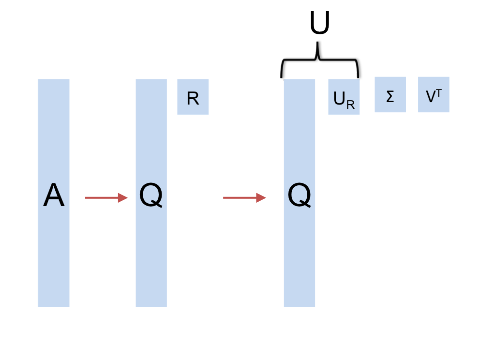
\includegraphics[height=6cm]{ur.png}

Bu demektir ki eğer $R$ üzerinde kütüphanemizin \verb!svd!  çağrısını
kullanırsak (ki $R$ nispeten ufak olduğu için bu ucuz olur) ele geçen $U_R$'i
alıp, $Q$ ile çarparsak, $A$ ayrıştırmasının $U$'sunu elde ederiz! $Q$ ile
paralel yapılabilir.

Tekrar paylaşmak gerekirse paralelleştirme teknikleri [6,8] yazılarında.

Kaynaklar

[1] Benson, A., {\em Tall-and-skinny Matrix Computations in MapReduce}

[2] Bayramlı, {\em Lineer Cebir Ders 22},
     \url{https://burakbayramli.github.io/dersblog/linear/linear_22/ders_22.html}

[3] Bayramlı, \url{https://burakbayramli.github.io/dersblog/sk/2022/11/paralel-lineer-cebir.html}     

[4] Bayramlı, Lineer Cebir, {\em Ders 29}

[5] Bayramlı, Lineer Cebir, {\em Matris Çarpımı, Ders 1}

[6] [Lineer Cebir ve Hadoop](https://burakbayramli.github.io/dersblog/sk/2015/03/lineer-cebir-hadoop.html)

[7] Zadeh, {\em CME 323: Distributed Algorithms and Optimization, Lecture 17},
    \url{https://stanford.edu/~rezab/classes/cme323/S17/}

[8] Bayramlı, {\em Paralel Lineer Cebir},
    \url{https://burakbayramli.github.io/dersblog/sk/2022/11/paralel-lineer-cebir.html}

[9] Gundersen, {\em Matrix Multiplication as the Sum of Outer Products},
    \url{https://gregorygundersen.com/blog/2020/07/17/matmul/}

\end{document}






